\documentclass[12pt, letterpaper]{article}
\usepackage{graphicx} %Latex package to import graphics (i.e. images)
\graphicspath{{etc}}
\title{Why is $ \frac{\partial J(W)}{\partial W_{i,j}^{(out)}} = (A^{(h)})^{T} \delta^{(out)}$ ?}
\author{Kassi Bertrand}
\date{January 2023}

\begin{document}
\maketitle

\section{Introduction}
In this \LaTeX{} document, I want to show my step-by-step process
to derive the partial derivative of all the weights in $W^{(out)}$.

\vspace{5mm} %5mm vertical space

I'll start simple with a 2-2-2 MLP, which is a Multi-Layer Perceptron
with 2 inputs, 2 hidden units, and 2 outputs, and then generalize
what we learn to a general $m-d-t$ MLP.

\vspace{5mm} %5mm vertical space

In both cases, I will use the following loss/error function:
\[J(w) = -\sum\nolimits_{i = 1}^{n}\sum\nolimits_{j=1}^{t} y_j^{[i]} ln(a_j^{[i]}) + (1 - y_j^{[i]})ln(1 - a_j^{[i]})\]

Where the superscript $[i]$ is an index for training examples,
and $j$ is the number of output units.

\vspace{5mm} %5mm vertical space

Ready? Let's go!

\pagebreak
\section{With a 2-2-2 MLP}

For this example, we will use the following Neural network:

%2-2-2 MLP picture
\begin{center}
    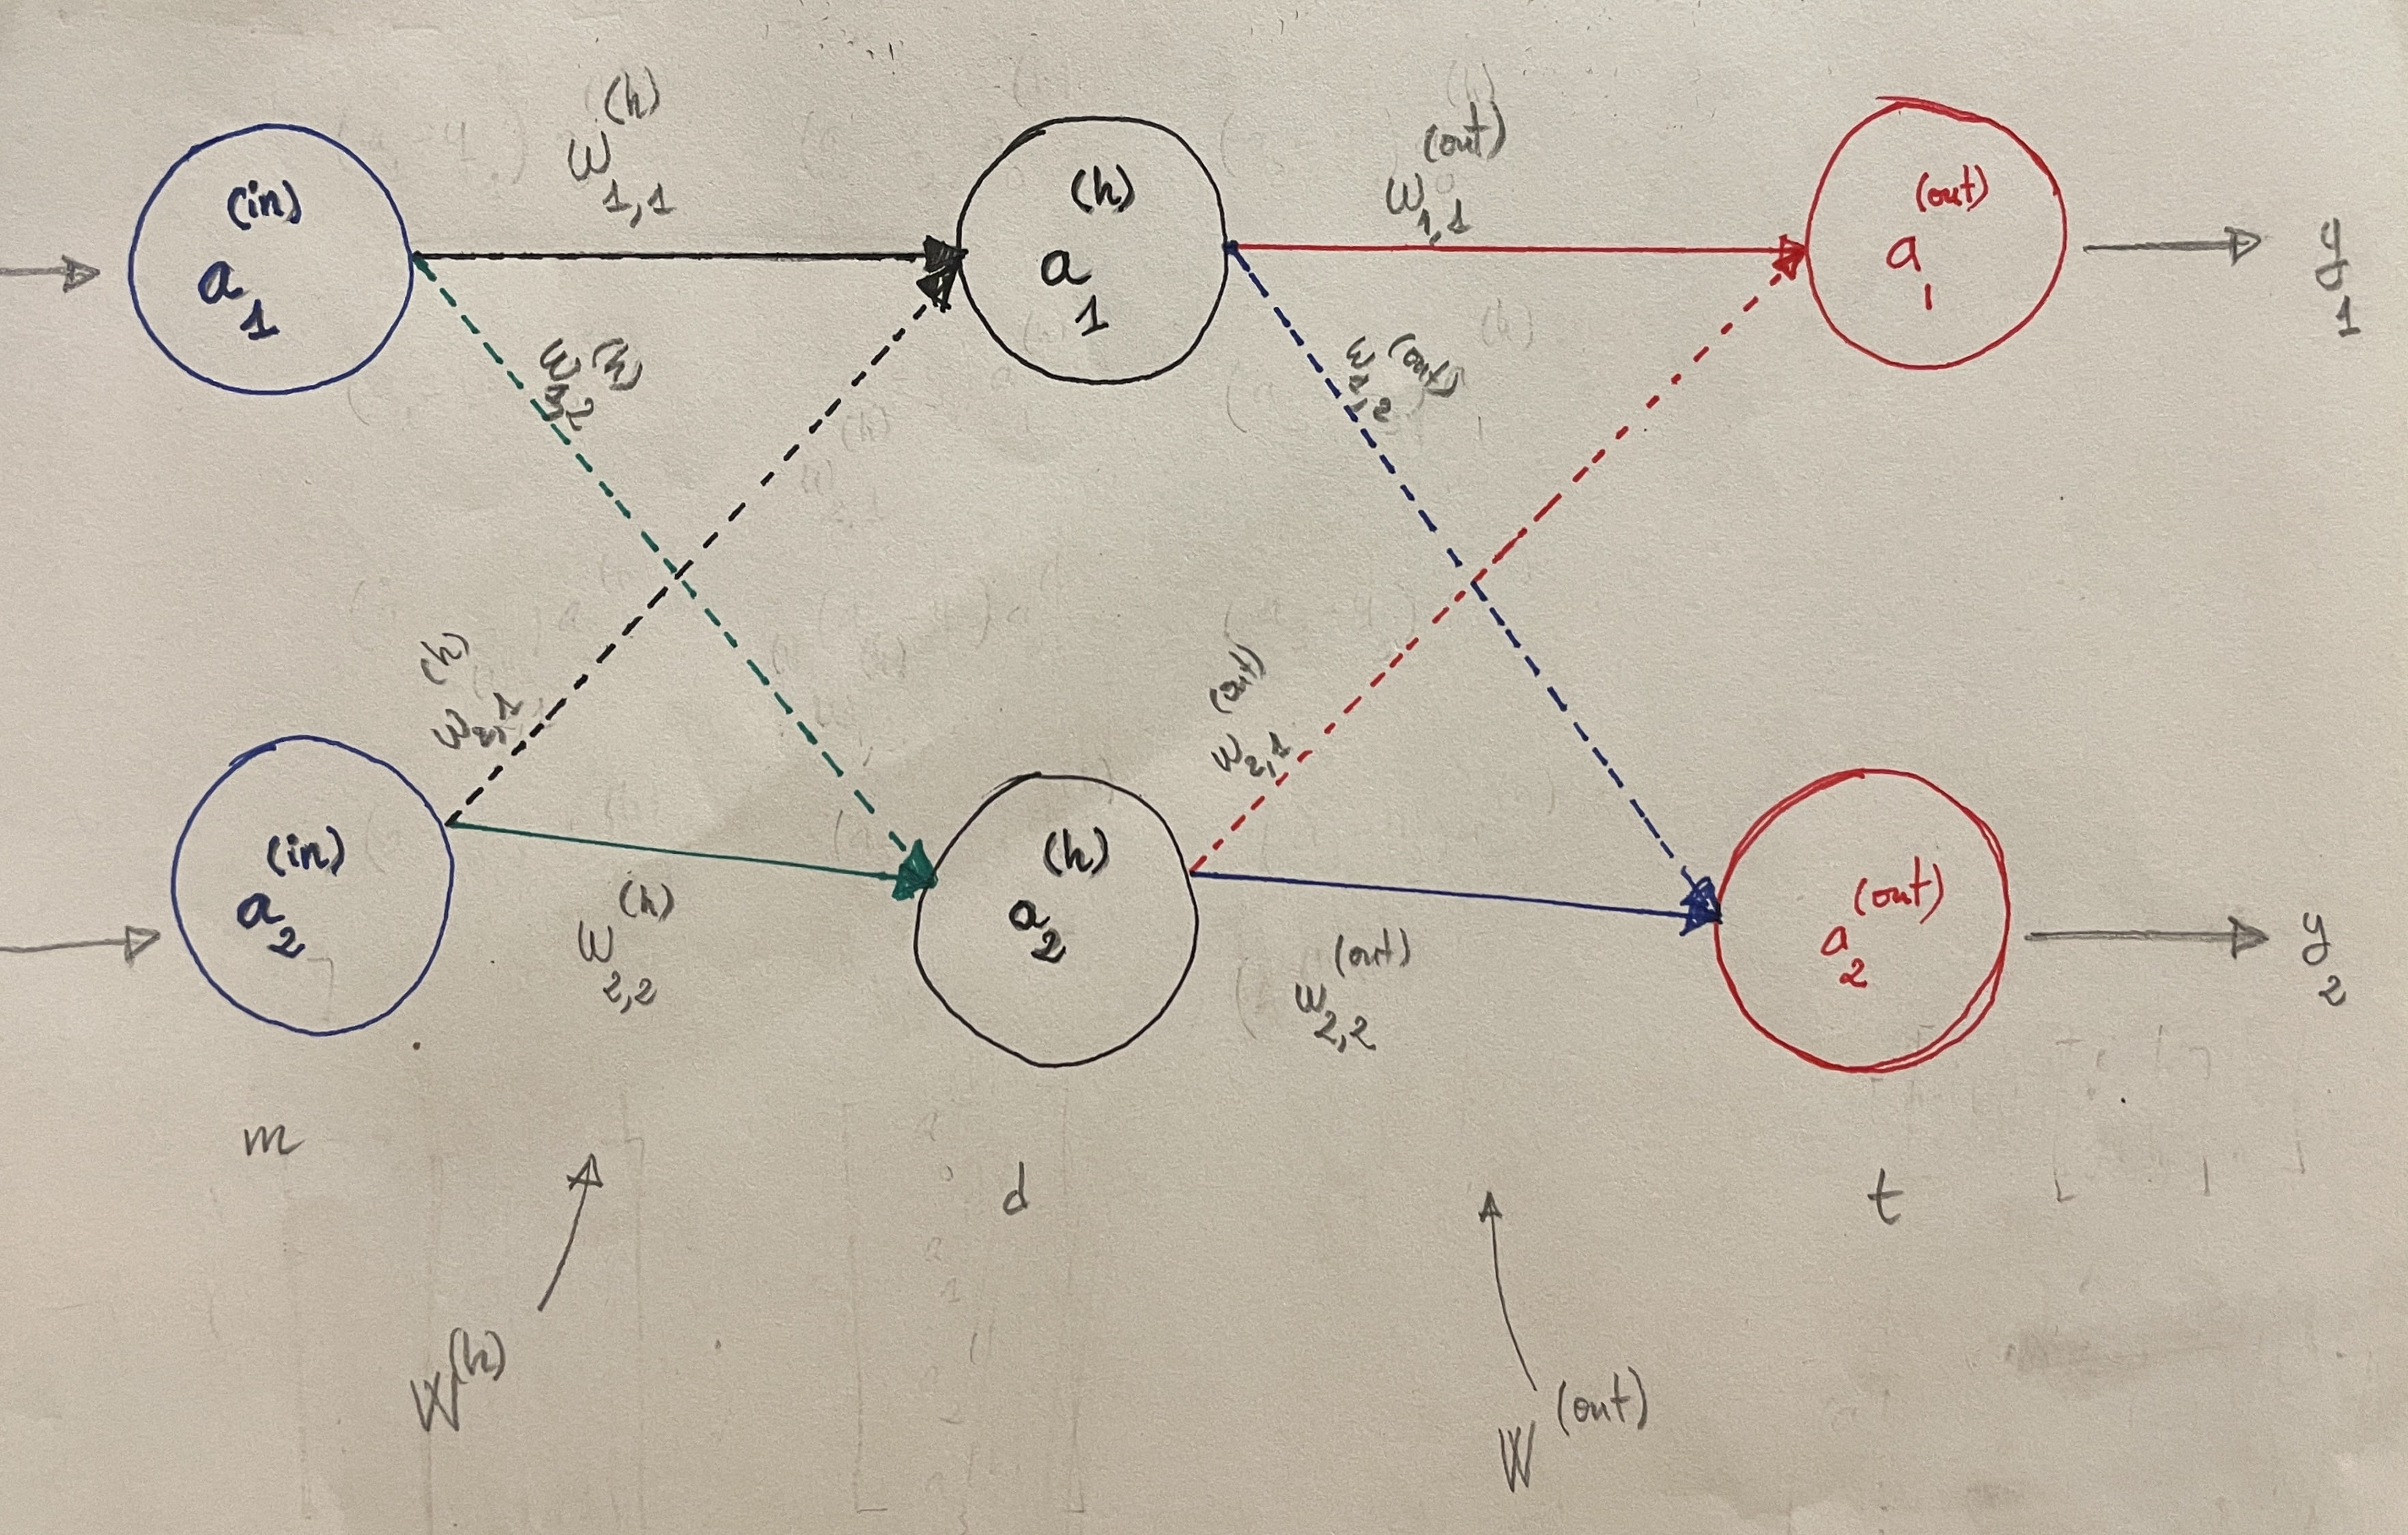
\includegraphics[width = 16cm, height = 9cm]{2-2-2-mlp.jpg}
\end{center}

\vspace{5mm} %5mm vertical space

We'll ignore biase units in the input and hidden layers, and 
consider only ONE training example for simplicity purposes.

\vspace{5mm} %5mm vertical space

Since one training example is considered and the network has
two output units, then  $n = 1$ and $t = 2$. So, the loss 
function becomes like this:

\[J(w) = -\sum\nolimits_{j=1}^{t} y_j^{[1]} ln(a_j^{[1]}) + (1 - y_j^{[1]})ln(1 - a_j^{[1]})\]

\vspace{5mm} %5mm vertical space

The journey of a SINGLE training example from the input layer to
the output layer goes like this:

\vspace{5mm} %5mm vertical space

\pagebreak
\[[a_1^{(in)}, a_2^{(in)}]\]
\[\downarrow\]
\[W^{(h)}\]
\[\downarrow\]                  
\[[z_1^{(h)}, z_2^{(h)}]\]
\[\downarrow\]
\[\phi(\bullet)\]
\[\downarrow\]
\[[a_1^{(h)}, a_2^{(h)}]\]
\[\downarrow\]
\[W^{(out)}\]
\[\downarrow\]                  
\[[z_1^{(out)}, z_2^{(out)}]\]
\[\downarrow\]
\[\phi(\bullet)\]
\[\downarrow\]
\[[a_1^{(out)}, a_2^{(out)}]\]

\section{With a general $m-d-t$ MLP}
\end{document}